%%%%%%%%%%%%%%%%%%%%%%%%%%%%%%%%%%%%%%%%%%%%%%%%%%%%%%%%%%%%%%%%%%%%%%%%%%%%%%%%%%%%%%%%%%%%%%%%%%%%%%
%
%   Filename    : chapter_5.tex 
%
%   Description : This file will contain your System Design.
%                 
%%%%%%%%%%%%%%%%%%%%%%%%%%%%%%%%%%%%%%%%%%%%%%%%%%%%%%%%%%%%%%%%%%%%%%%%%%%%%%%%%%%%%%%%%%%%%%%%%%%%%%

\chapter{System Design}

\section{System Overview}
FireflyX is a mobile application tool that aims to aid children in learning music fundamentals. There will only be one role, which is the user. The target users are children of ages 5 to 8 with little knowledge of music. The user may edit the firefly models' parts based on their preferences.

The properties of the rhythm that can be configured on the firefly model are the tempo, length of the note, repetitions, rest pattern, and pitch. Each part of the firefly model directly corresponds to one property that can be modified.

The parts of the firefly model may be configured either by part or by manipulating the parts by gestures, such as pinching, swiping, and tapping. After a firefly model is configured, the user may set it free on a canvas where they can freely fly and roam. The rhythm will then be played with the properties set by the different parts the user has chosen or have tweaked. 

In order to create a rhythm, the user is allowed to make more firefly models with different configuration. The user will be allowed to play, pause, reset, stop, and save their current workspace.

\section{System Objectives}
The system aims to accomplish the following:
\begin{itemize}
    \item To enable users to make a rhythm and pitch using firefly models.
    \item To allow users to change the properties of the rhythm and pitch by tweaking the parts of the firefly model.
    \item To allow users to start playback by releasing the firefly models.
    \item To allow users to access previous tracks using a playback history.
    \item To allow users to save and load their current workspace.
\end{itemize}
\section{System Scope and Limitations}
The users can make rhythms by modifying the firefly models. We will only include rhythms and pitch, specifically claps and rests, no harmonies. The properties of the music can be modified by tweaking the parts of the firefly model.

The tempo of the firefly model can be chosen by the changing the body model. The body will be including only the 7 tempos used namely \textit{grave, allegro, larghetto, moderato, andante, adagio,} and \textit{largo}. The wing speed can be set by buttons to change the length of the note. The slower wing will represent slower notes and the faster wing will represent faster notes. For setting the repetition of the pattern, the wing size can be selected. The bigger sized wings will represent more repetitions, and the smaller sized wings will represent less repetitions. The speed and sizes will only be integers. The light of the firefly model is the pattern for the rests of the note. The number of patterns can be seen in Table \ref{Patterns}. Also the pitch will be represented by the biscuits scattered in the environment. 

Each workspace will be considered as an album. The user is given five fireflies in jar to play with. After the user modifies the firefly models, they can be released outside the jar. Only five fireflies may roam outside freely, where the firefly will traverse through a trail which leads to it moving to another note's pitch. After the fireflies that are currently playing are finished, they will be automatically be saved as a track. The track will be added to the album track list. The track will be represented also as a jar.

The users will be able to listen to previous tracks by using a playback history. The playback history is a list of jars that can be found under the playback controls.  

The users are allowed to save their current workspace. The saved file will include the current album, track list, and the configurations of the fireflies. An XML file format will be used for the saved files. These saved data can be loaded by the user at any time. Each save will ask the input for the title and author.

\section{Architectural Design}

\begin{figure} [H]
    \centering
    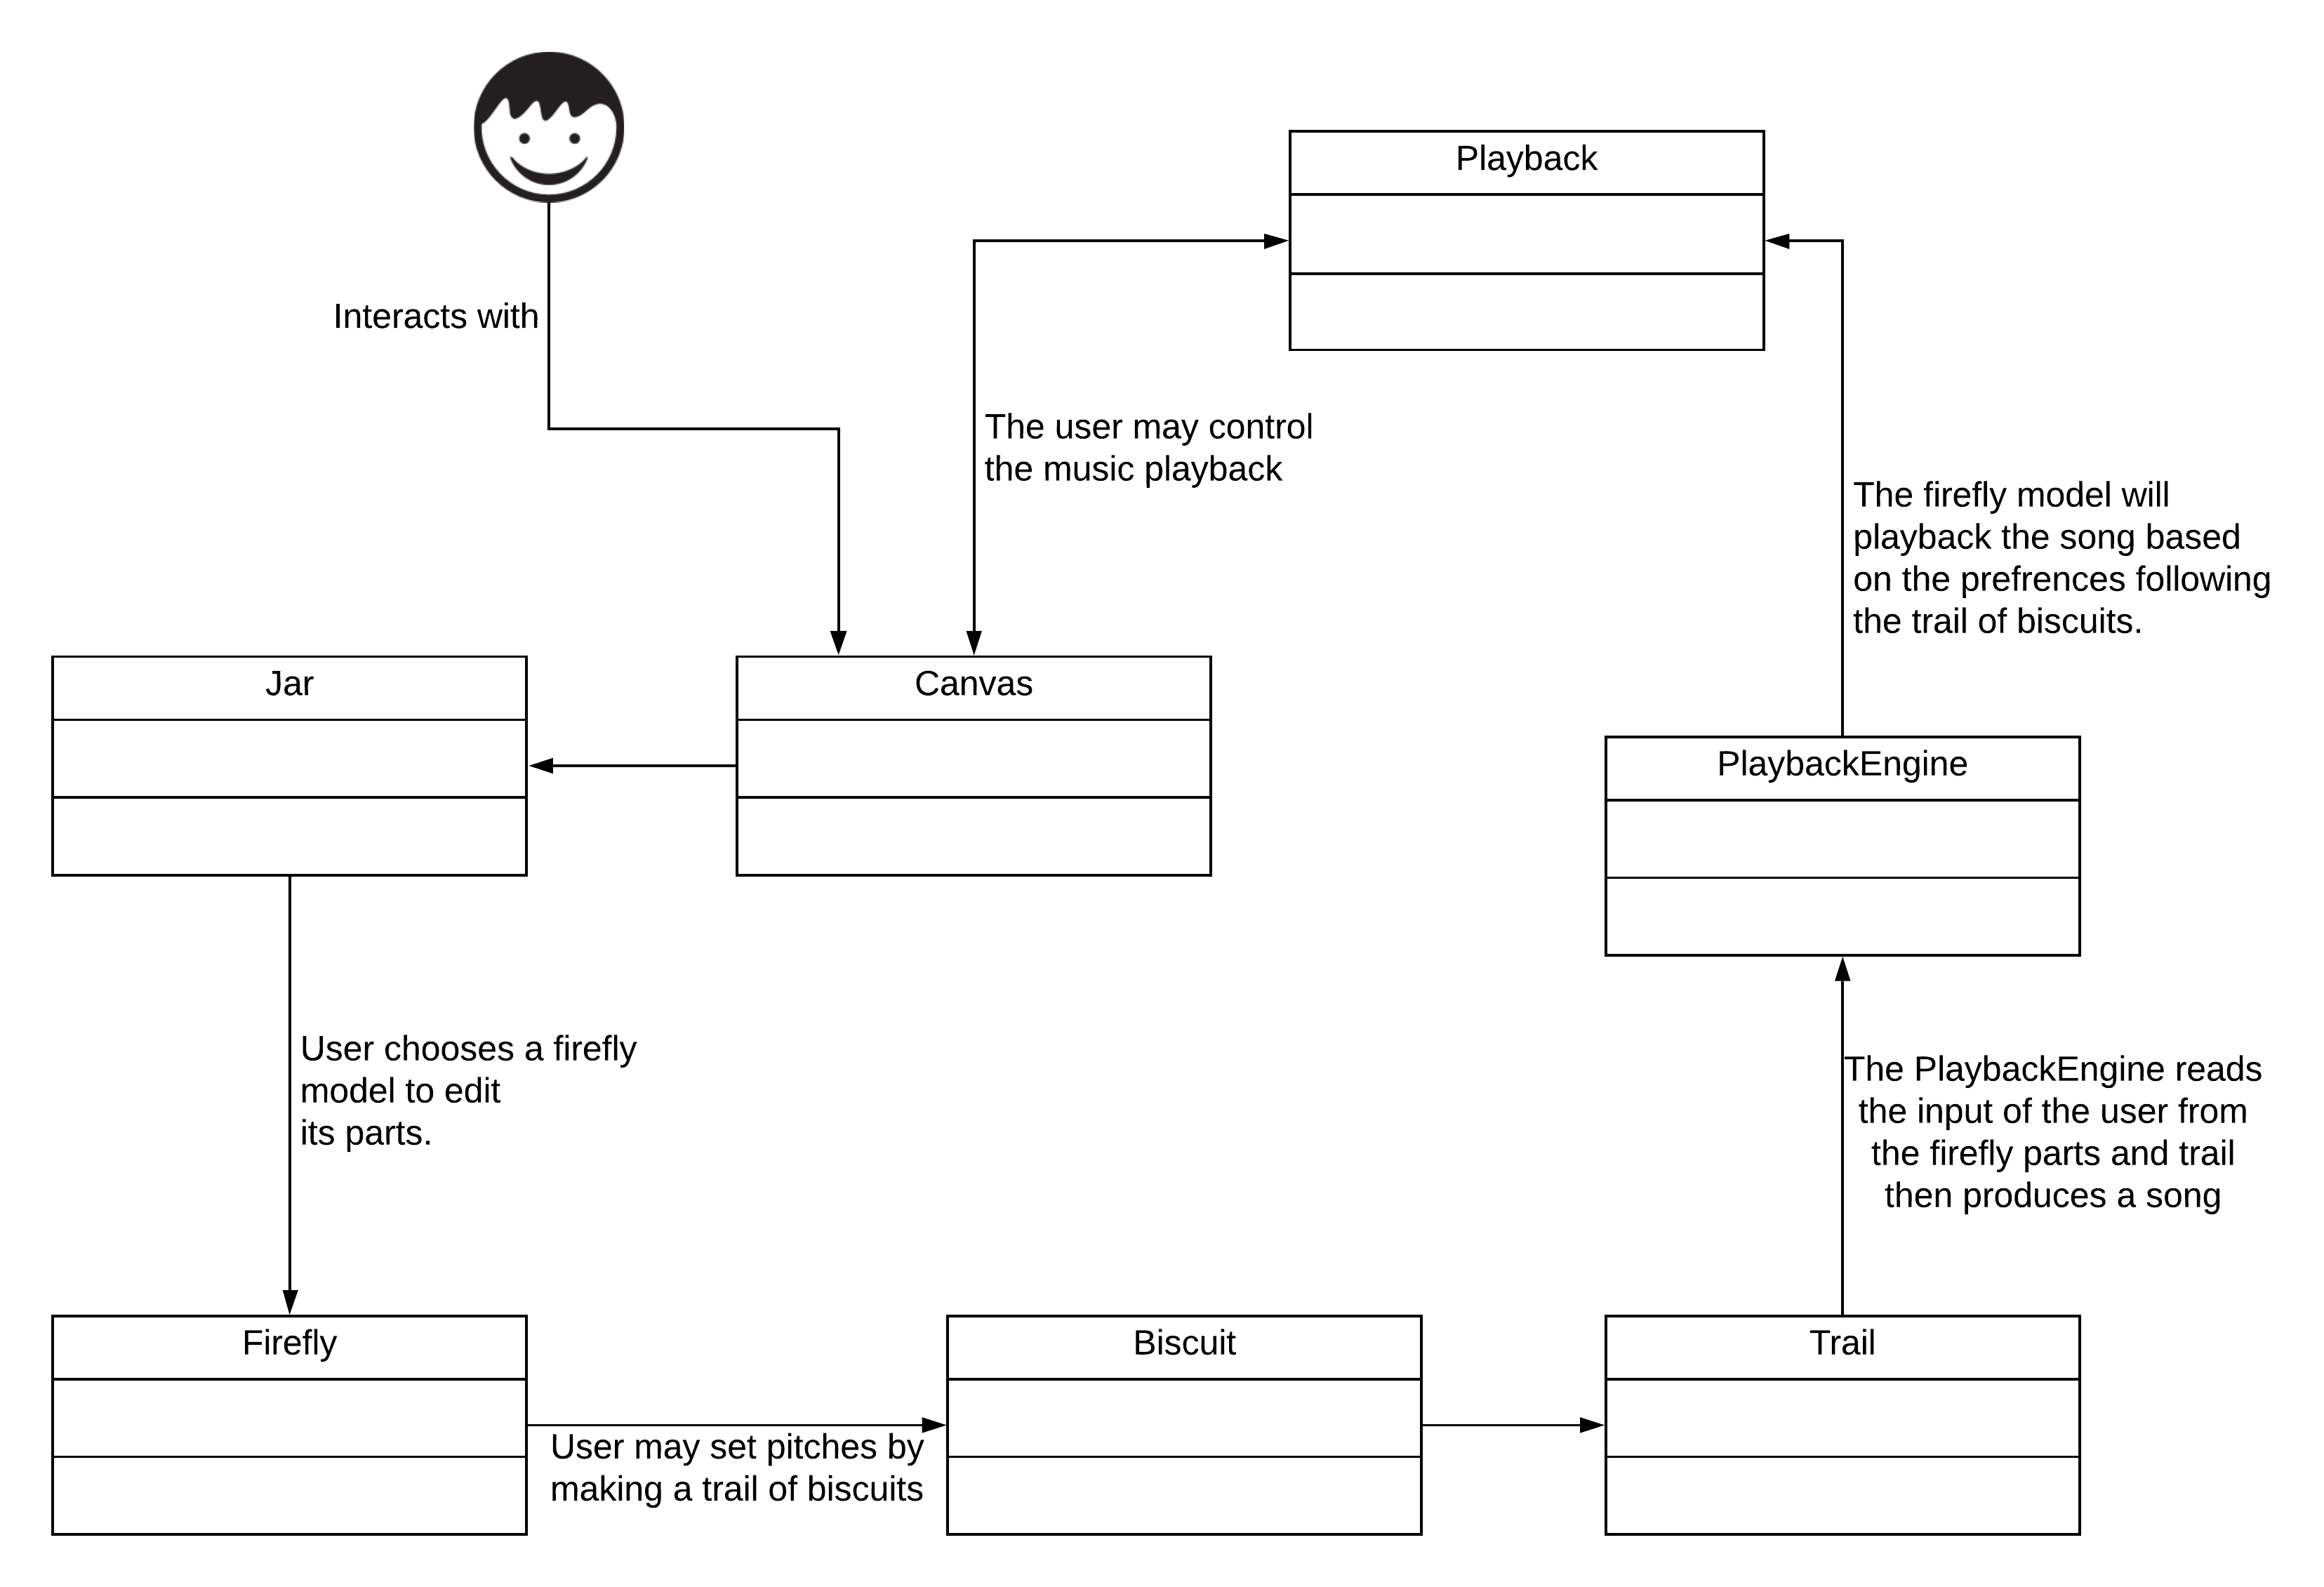
\includegraphics[width=15cm]{figures/NewSysArchi.png}
    \caption{The System Architecture of FireflyX}
    \label{fig:sysarchi}
\end{figure}

\begin{figure} [H]
    \centering
    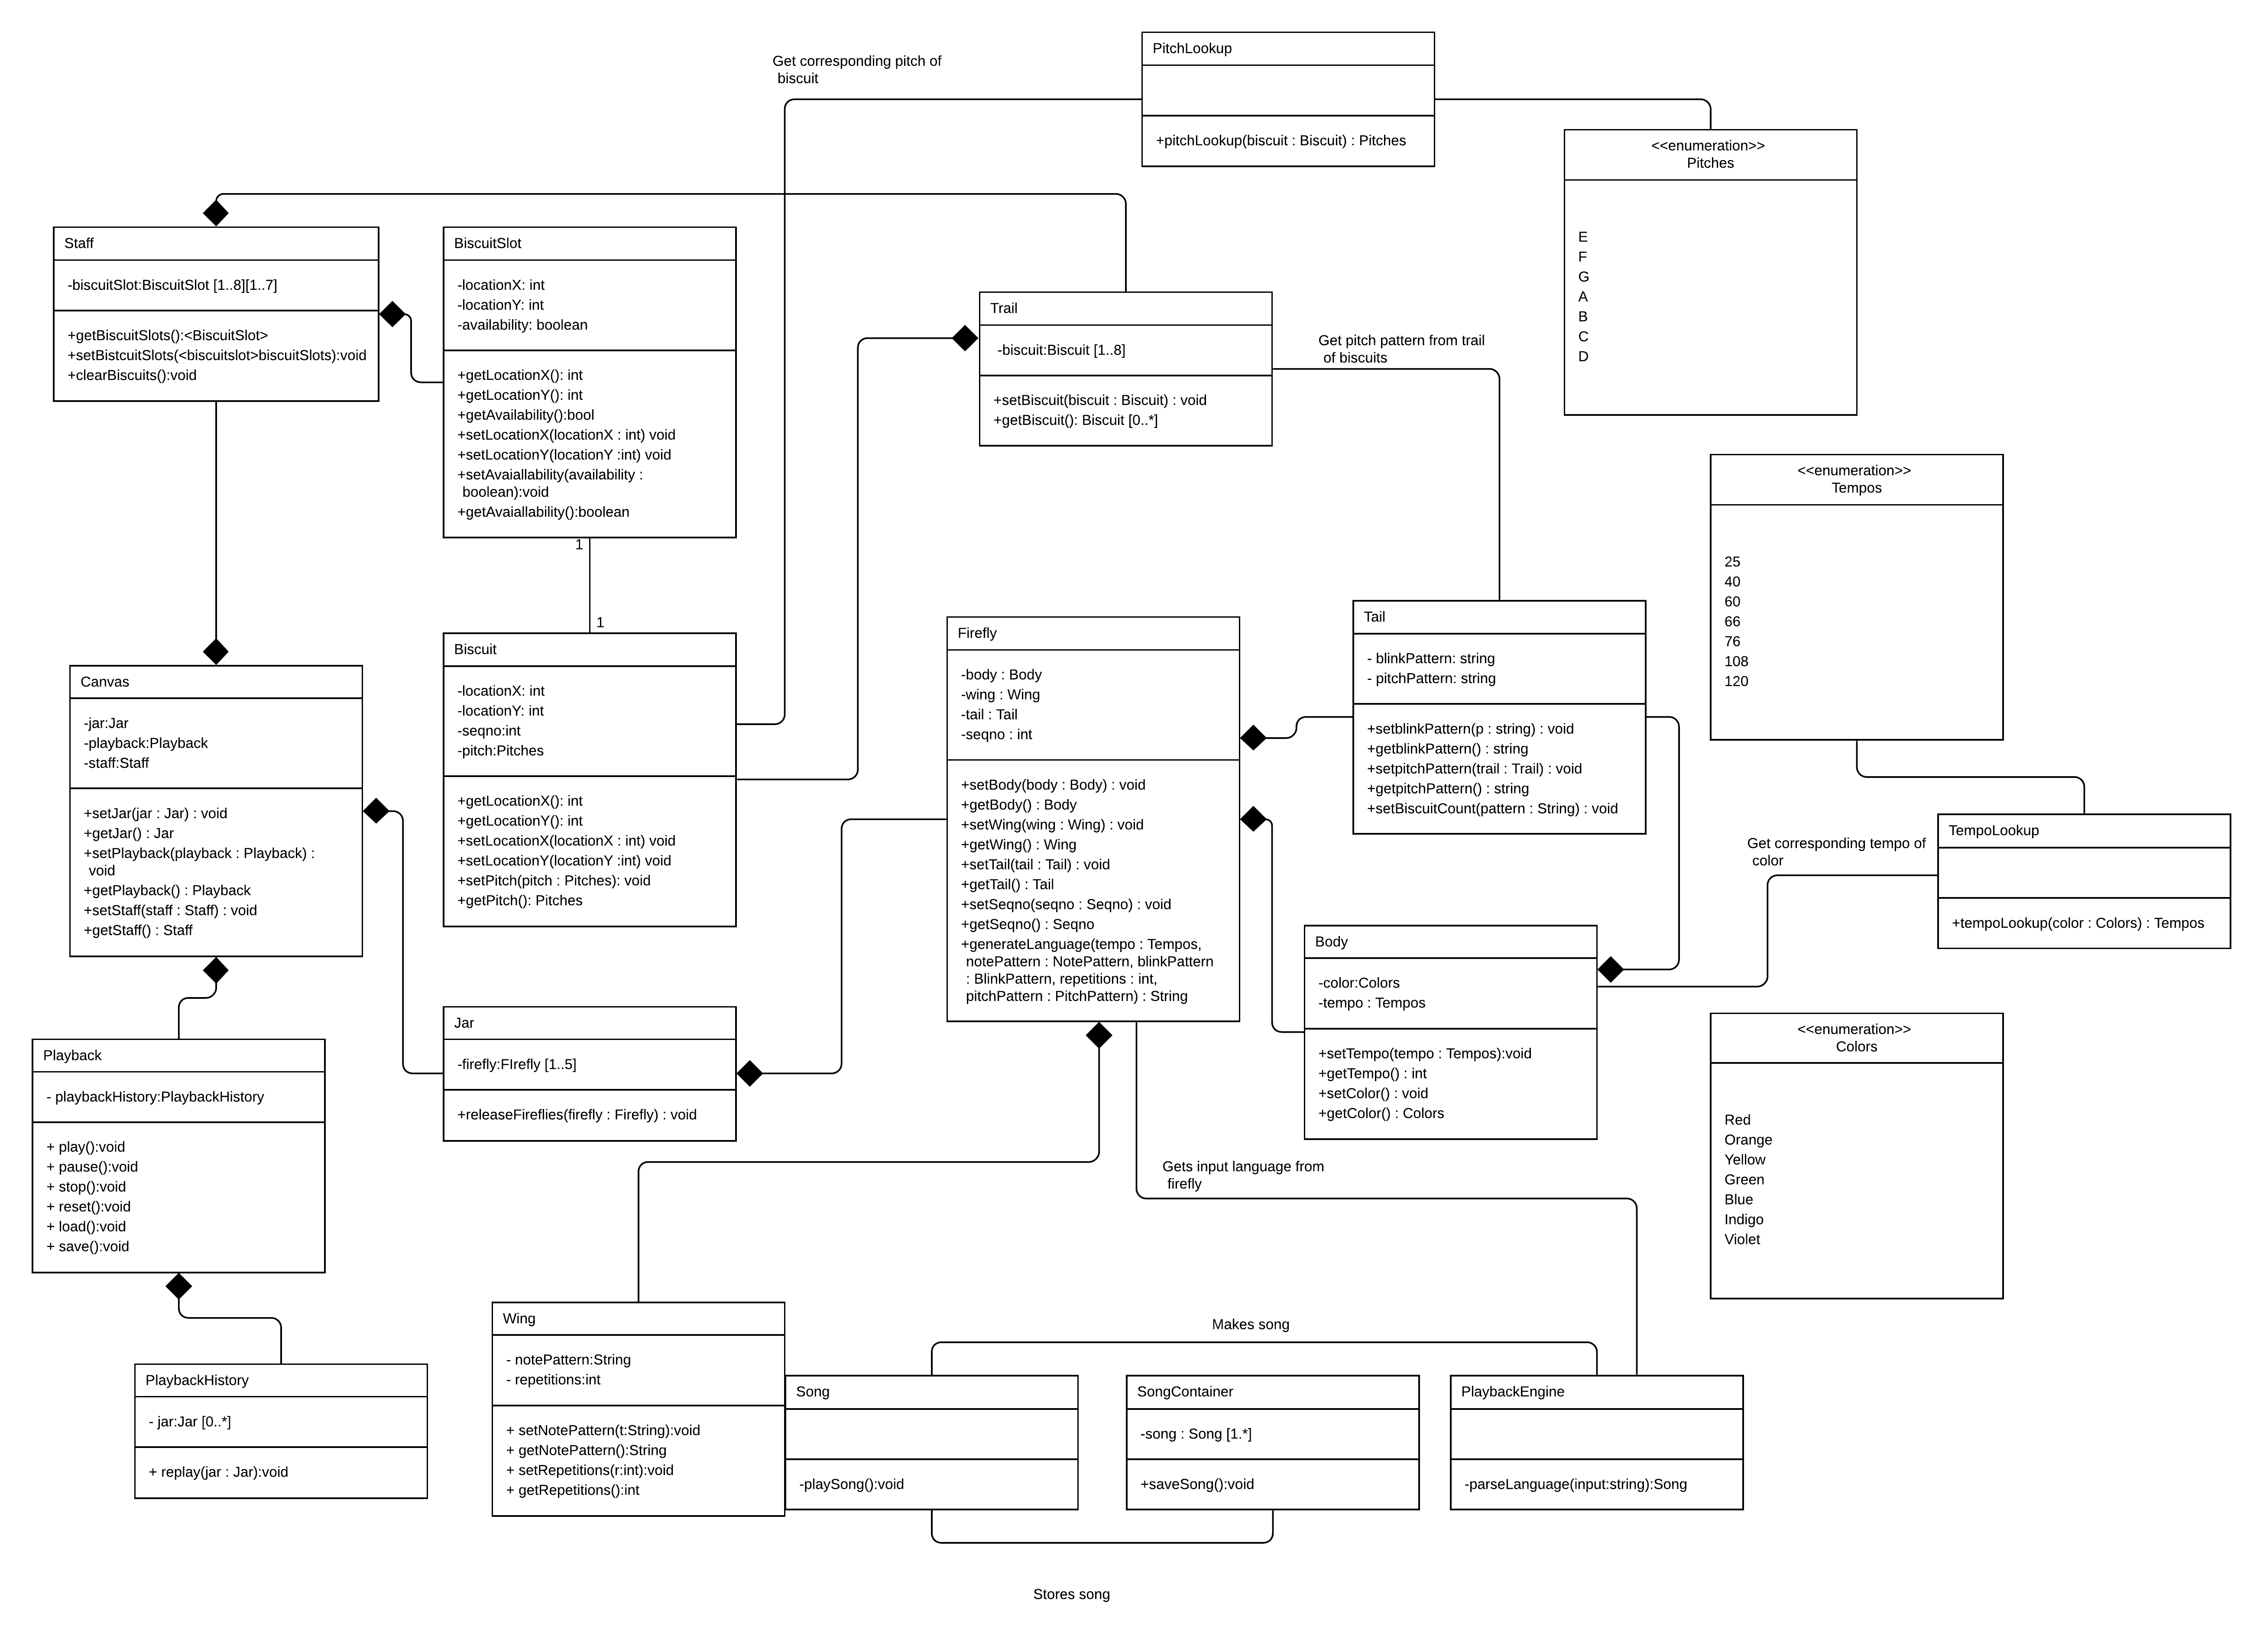
\includegraphics[width=17cm]{figures/FireflyXUML.png}
    \caption{UML Class Diagram of FireflyX}
    \label{fig:fireflyxUML}
\end{figure}

Figure \ref{fig:sysarchi} and Figure \ref{fig:fireflyxUML} shows the architecture of the system. The system follows a Model-View-Controller architecture. All processes will be handled locally by the device. Figure \ref{fig:fireflyxUML} shows the detailed class diagrams for the system.
    
\section{System Features}
The following are the features of the FireflyX application. Features such as firefly model parts popup settings, playback toolbox, jar sandbox environment, and the canvas.

% \subsection{Firefly Parts Toolbox}
% The toolbox serves to give the user the parts needed to make the firefly. The toolbox includes the head, body, wings, and the tails. Assembling different fireflies have different musical properties. These properties can be fine tuned using this toolbox. The chosen parts will correspond to a string of rhythm pattern language that will be parsed by our playback module when the firefly is released to the sandbox environment.

\subsubsection{Body Popup Settings}
The body section of the firefly model can be tapped to show the popup settings. In the popup settings of the body section, the user is able to choose the tempo of the taps that the firefly will play. Each unique color of the body has an equivalent tempo. The user can also scroll through a variety of body models. The preferences of the body will be appended to the string of rhythm pattern language. For every environment once a body has been set for the first firefly the succeeding fireflies will have the same color with the first and by changing one the others get changed as well.

\subsubsection{Wings Popup Settings}
The wing section of the firefly model can be tapped to show the popup settings. In the popup settings of the wings section, the user is able to choose the speed of the note being played by pressing 1, 2, 4, or 8 which represents the whole note, half note, quarter note, eighth note, respectively. The size of the wing will represent the number of repetitions. The minimum size is 1 and the maximum size is 6. The wing preferences will be appended to the string of rhythm pattern language.

\subsubsection{Tail Light Popup Settings}
The tail section of the firefly model can be tapped to show the popup settings. On the right side, the user is able to change the rest pattern of the note being played. The tail lights will be blinking patterns and pattern can be previewed in popup settings, the light will be based from the chosen color in the body. The patterns will be predetermined by our library of patterns. The left side will be a button for setting the pitch. The chosen pattern will be appended to the string of rhythm and pitch pattern language.

\subsubsection{Set Pitch Mode}
The mode is only accessible upon tapping the feed me button. The feed me button can be accessed during the tail pop settings. There will be a staff where the biscuits may be placed. The biscuits will be representing the notes. The number of biscuits will depend on the number of claps in the chosen pattern. The placement of the notes will also be determining the flight pattern of the firefly model. The preview button will also act like a playback for one specific firefly. The clear button will allow the user to reset the biscuits. The chosen pitch pattern will be appended to a separated pattern language.

\subsection{Jar Sandbox Environment}
The sandbox environment will be represented by a jar. In the jar, five firefly models can be seen where each can be tapped. When a firefly model is tapped, it enlarges and enables the popup settings when a specific part is tapped. The cork can also be tapped to release all of the firefly models into the canvas.

\subsection{Canvas}
Once the jar lid is tapped, the finished firefly models are released into the canvas where they roam around and play music based on their settings by sequence. Once the firefly models on the canvas are done playing they will be automatically be added to the album track list.

\subsection{Playback Control}
This toolbox will allow the user to control the playback of the firefly models. The user may pause, play, stop, and mute the music playback at anytime by clicking the play, pause, stop, and mute icons in the toolbox. The user is also able to save the existing workspace, and load a saved workspace. This can be done by clicking the save, and load buttons respectively. The user is also able to view previous tracks. In order to see the previous tracks, there will be a track list at the playback toolbox. The volume of the playback can be controlled by the slider on top of the canvas. Sliding to the sun means higher volume, and sliding to the moon means lower volume.


\section{Music Language, Rules and Library of Patterns}

\begin{table}[H]
\caption{Rhythm Representation}
\label{musiclang}
\centering
\begin{tabular}{|l|l|r|} 
\hline
Note Representation & Music Notation & Integer Equivalent  \\ 
\hline
W                   & Whole Note     & 1                   \\ 
\hline
H                   & Half Note      & 2                   \\ 
\hline
Q                   & Quarter Note   & 4                   \\ 
\hline
E                   & Eighth Note    & 8                   \\ 
\hline
Wr                  & Whole Rest     & -1                  \\ 
\hline
Hr                  & Half Rest      & -2                  \\ 
\hline
Qr                  & Quarter Rest   & -4                  \\ 
\hline
Er                  & Eighth Rest    & -8                  \\
\hline
\end{tabular}
\end{table}

\begin{table}[H]
\caption{Pitch Representation}
\label{pitchRep}
\centering
\begin{tabular}{|l|l|r|} 
\hline
Pitch of Note & Pitch Representation   \\ 
\hline
A                   & (a)                     \\ 
\hline
B                   & (b)                      \\ 
\hline
C                   & (c)                      \\ 
\hline
D                   & (d)                    \\ 
\hline
E                   & (e)                      \\ 
\hline
F                   & (f)                       \\ 
\hline
G                   & (g)                    \\ 
\hline
Rest                   & (-)                    \\ 
\hline
\end{tabular}
\end{table}

\begin{table}[H]
\caption{Tempo Representation}
\label{pitchRep}
\centering
\begin{tabular}{|l|l|r|} 
\hline
Name of Tempo & Beats Per Minute   \\ 
\hline
Grave                  & 25 bpm                     \\ 
\hline
Largo                  & 40 bpm                      \\ 
\hline
Larghetto                  & 60 bpm                      \\ 
\hline
Adagio                  & 66 bpm                    \\ 
\hline
Andante                   & 76 bpm                      \\ 
\hline
Moderato                   & 108 bpm                       \\ 
\hline
Allegro                  & 120 bpm                    \\ 
\hline
\end{tabular}
\end{table}

To help us better understand the music sheets from the Book 1 of the Suzuki teaching method, we decided to convert the sheets to a language we can easily understand and represent on code. See Table \ref{musiclang} for reference to the converted language. This will mainly be used for the representation for the first iteration since at this iteration it only covers rhythm. To make the app easier to use, a set of rules for the music composition has been used. The firefly will only be using a maximum of 6 measures per rhythm. Each measure is equal to 1 pattern. The speed of the notes and rests that will be supported by the application will only be the whole, half, quarter, and eighth note.

The following patterns are taken from the Book 1 of the Suzuki teaching method, included here are the 3 most common clap and rest patterns found in each clap and rest combination (see Table \ref{Patterns}). For the representation in the table, 1 is for the clap and the 0 is for the rest. An example as seen from the table is "1Rest" - the number 1 coefficient represents the number of instances of the rest. A change in pattern from rest to tap is separated by a dash. 

For iteration two and three since pitch will already be added we would use the same set of patterns and add a corresponding pitch to a note denoted inside a parenthesis from the seven pitches found in Table \ref{pitchRep} and also how to represent ones from a rest. An example pattern is shown through two sample pieces of music (found in Appendix \ref{sec:appendixe}), the sample representation is seen in Table \ref{PitchPatterns}.

\begin{landscape}
\begin{table}
\centering
\caption{Common Patterns in Suzuki Book 1}
\label{Patterns}
\begin{tabular}{|l|l|l|l|} 
\hline
 \textbf{Pattern}                                                                                                                                                              & \textbf{Pattern Name}                                                                                                                                                                                                    & \textbf{Count}                                                                                                                                                  & \textbf{Pattern Note Count}                                                                                                                                                                                                                \\ 
\hline
\begin{tabular}[c]{@{}l@{}}0 \\\\1\end{tabular}                                                                              & \begin{tabular}[c]{@{}l@{}}1Rest \\\\1Clap\end{tabular}                                                                                                                & \begin{tabular}[c]{@{}l@{}}23\\\\1\end{tabular}                                                               & \begin{tabular}[c]{@{}l@{}}{[}Wr - 23] \\\\{[}W - 1]\end{tabular}                                                                                                                        \\ 
\hline
\begin{tabular}[c]{@{}l@{}}001\\ \\ 010\\ \\ 100\end{tabular}              & \begin{tabular}[c]{@{}l@{}}2Rest-1Clap\\ \\ 1Rest-1Clap-1Rest\\ \\ 1Clap-2Rest \end{tabular}                         & \begin{tabular}[c]{@{}l@{}}12\\ \\ 6\\ \\ 2 \end{tabular}   & \begin{tabular}[c]{@{}l@{}}HrQrQ - 12]\\ \\ {[}QrQHr - 5, HrQQr - 1]\\ \\ {[}QQrHr - 2] \end{tabular}                                  \\ 
\hline
\begin{tabular}[c]{@{}l@{}}1010\\ \\ 1111\\ \\ 1110 \end{tabular}          & \begin{tabular}[c]{@{}l@{}}1Clap-1Rest-1Clap-1Rest\\ \\ 4Clap\\ \\ 3Clap-1Rest \end{tabular}                         & \begin{tabular}[c]{@{}l@{}}39\\ \\ 22\\ \\ 5 \end{tabular}  & \begin{tabular}[c]{@{}l@{}}QQrQQr - 39] \\ \\ {[}QQQQ - 21, EEQH - 1]\\ \\ {[}QQQQr - 5] \end{tabular}                                 \\ 
\hline
\begin{tabular}[c]{@{}l@{}}10110\\ \\ 11111\\ \\ 01101 \end{tabular}       & \begin{tabular}[c]{@{}l@{}}1Clap-1Rest-2Clap-1Rest\\ \\ 5Clap\\ \\ 1Rest-2Clap-1Rest-1Clap \end{tabular}             & \begin{tabular}[c]{@{}l@{}}26\\ \\ 10\\ \\ 13 \end{tabular} & \begin{tabular}[c]{@{}l@{}}QQrEEQr - 26]\\ \\ {[}QEEQQ -4, QQQEE -3, EQEQQ- 1, EEQQQ -1, EQQQE -1]\\ \\ {[}QrEEQrQ -13] \end{tabular}  \\ 
\hline
\begin{tabular}[c]{@{}l@{}}110110\\ \\ 111111\\ \\ 011011 \end{tabular}    & \begin{tabular}[c]{@{}l@{}}2Clap-1Rest-2Clap-1Rest\\ \\ 6Clap\\ \\ 1Rest-2Clap-1Rest-2Clap \end{tabular}             & \begin{tabular}[c]{@{}l@{}}20\\ \\ 3\\ \\ 6 \end{tabular}   & \begin{tabular}[c]{@{}l@{}} EEQrEEQr - 20 ]\\ \\ {[} EEQEEQ - 2, QQEQQE - 1 ]\\ \\ {[} QrEEQrEE - 6 ] \end{tabular}                    \\ 
\hline
\begin{tabular}[c]{@{}l@{}}1111111\\ \\ 0101011\\ \\ 0111011~\end{tabular} & \begin{tabular}[c]{@{}l@{}}7Clap\\ \\ 1Rest-1Clap-1Rest-1Clap-1Rest-2Clap\\ \\ 1Rest-3Clap-1Rest-2Clap \end{tabular} & \begin{tabular}[c]{@{}l@{}}14\\ \\ 4\\ \\ 2 \end{tabular}   & \begin{tabular}[c]{@{}l@{}} EEEEEEQ - 11, EEQEEEE - 3 ]\\ \\ {[} ErEErEErEQ - 4 ]\\ \\ {[} ErEEEErEQ - 2 ] \end{tabular}               \\ 
\hline
\begin{tabular}[c]{@{}l@{}}11110110\\ \\ 11111111 \end{tabular}                                                              & \begin{tabular}[c]{@{}l@{}}4Clap-1Rest-2Clap-1Rest\\ \\ 8Clap \end{tabular}                                                                                            & \begin{tabular}[c]{@{}l@{}}4\\ \\ 3 \end{tabular}                                                             & \begin{tabular}[c]{@{}l@{}}EEEEErEEEr - 4 ]\\ \\ {[}EEEEEEEE - 3 ] \end{tabular}                                                                                                         \\
\hline
\end{tabular}
\end{table}
\end{landscape}

\begin{table}
\centering
\caption{Patterns Found in Hot Cross Buns and Old Macdonald}
\label{PitchPatterns}
\begin{tabular}{|l|l|l|l|} 
\hline
 \textbf{Pattern }                                                                                     & \textbf{Pattern Name}                                                                                          & \textbf{Count}                                                                                   & \textbf{Pattern Note Count (with Pitch)}                                                                                                         \\ 
\hline
0                                                                                                      & 1Rest                                                                                                          & 1                                                                                                & {[}Wr(-) - 1]                                                                                                                                    \\ 
\hline
10                                                                                                     & 1Clap-1Rest                                                                                                    & 1                                                                                                & {[}H(g)Hr(-) - 1]                                                                                                                                \\ 
\hline
111                                                                                                    & 3Clap                                                                                                          & 3                                                                                                & {[}Q(b)Q(a)H(g) - 3]                                                                                                                             \\ 
\hline
\begin{tabular}[c]{@{}l@{}}1110\\\\1111\end{tabular} & \begin{tabular}[c]{@{}l@{}}3Clap-1Rest\\\\4Clap\end{tabular} & \begin{tabular}[c]{@{}l@{}}1\\\\1\end{tabular} & \begin{tabular}[c]{@{}l@{}}{[}Q(g)Q(g)Q(g)Qr(-) - 1]\\\\{[}Q(b)Q(b)Q(a)Q(a) - 1]\end{tabular}  \\ 
\hline
11111111                                                                                               & 8Clap                                                                                                          & 1                                                                                                & {[}E(b)E(b)E(b)E(b)E(a)E(a)E(a)E(a)]                                                                                                             \\
\hline
\end{tabular}
\end{table}

\section{Data Design}
Each selection of the firefly body part corresponds to an integer that references into a music library to get the necessary music files needed for the playback. The chosen format for the save files will be using XML. The file will be saving all the configurations of the current fireflies on the canvas. The file can be loaded and it will load the fireflies with their configurations that were saved on the file. The saved files will be stored locally on the device. Allowed inputs for the files can be seen in the table below in Table 5.6. An example xml file is also shown in Table \ref{XML} that shows how the sample piece Hot Cross Buns seen in Appendix \ref{sec:appendixe} will be saved.

% \begin{figure}[H]
%     \centering
%     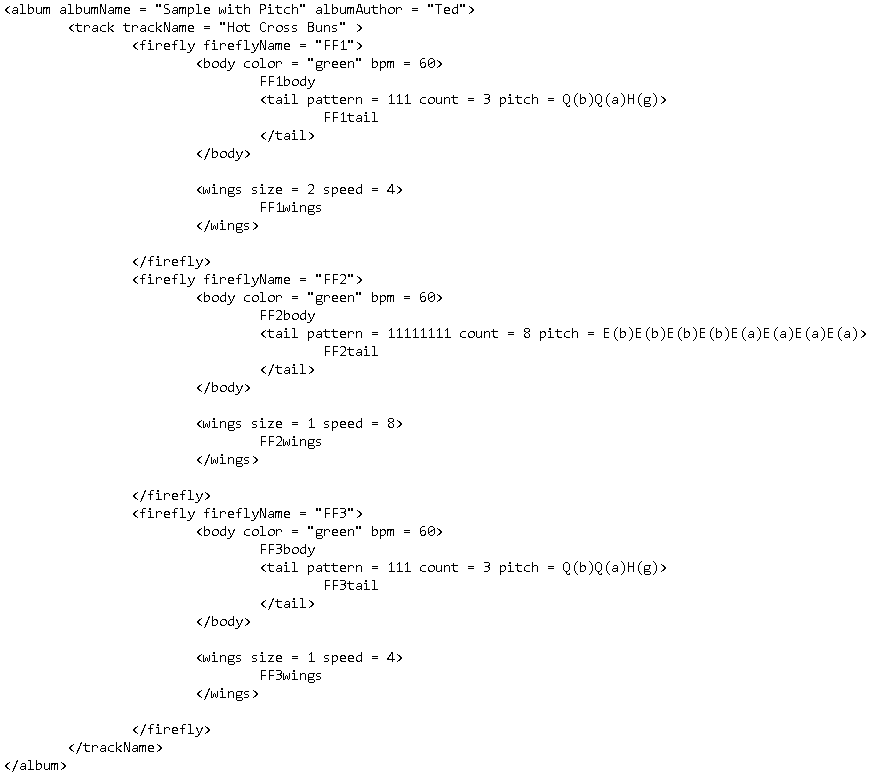
\includegraphics[width=17.6cm]{figures/sampleXML.png}
%     \caption{Sample XML}
%     \label{sampleXML}
% \end{figure}

\begin{landscape}
\begin{table}
\centering
\caption{Data Design Specifics}
\label{XML}
\begin{tabular}{|l|} 
\hline
\begin{tabular}[c]{@{}l@{}}\textless{}album albumName = "Sample with Pitch" albumAuthor = "Ted"\textgreater{}	albAlbum1						\\~ ~ ~ ~ \textless{}track trackName = "Hot Cross Buns" \textgreater{}	trkTrack1					\\~ ~ ~ ~ ~ ~ ~ ~ \textless{}firefly fireflyName = "ffObj1"\textgreater{}					\\~ ~ ~ ~ ~ ~ ~ ~ ~ ~ ~ ~ \textless{}body color = "green" bpm = 60\textgreater{}	ffObj1Body			\\~ ~ ~ ~ ~ ~ ~ ~ ~ ~ ~ ~ ~ ~ ~ ~ \textless{}tail pattern = 111 count = 3 pitch = Q(b)Q(a)H(g)\textgreater{}	ffObj1Tail		\\~ ~ ~ ~ ~ ~ ~ ~ ~ ~ ~ ~ ~ ~ ~ ~ \textless{}/tail\textgreater{}			\\~ ~ ~ ~ ~ ~ ~ ~ ~ ~ ~ ~ \textless{}/body\textgreater{}				\\~ ~ ~ ~ ~ ~ ~ ~ ~ ~ ~ ~ \textless{}wings size = 2 speed = 4\textgreater{}	ffObj1Wings			\\~ ~ ~ ~ ~ ~ ~ ~ ~ ~ ~ ~ \textless{}/wings\textgreater{}\\~ ~ ~ ~ ~ ~ ~ ~ \textless{}/firefly\textgreater{}					\\~ ~ ~ ~ ~ ~ ~ ~ \textless{}firefly fireflyName = "ffObj2"\textgreater{}					\\~ ~ ~ ~ ~ ~ ~ ~ ~ ~ ~ ~ \textless{}body color = "green" bpm = 60\textgreater{}	ffObj2Body			\\~ ~ ~ ~ ~ ~ ~ ~ ~ ~ ~ ~ ~ ~ ~ ~ \textless{}tail pattern = 11111111 count = 8 pitch = E(b)E(b)E(b)E(b)E(a)E(a)E(a)E(a)\textgreater{}	ffObj2Tail		\\~ ~ ~ ~ ~ ~ ~ ~ ~ ~ ~ ~ ~ ~ ~ ~ \textless{}/tail\textgreater{}			\\~ ~ ~ ~ ~ ~ ~ ~ ~ ~ ~ ~ \textless{}/body\textgreater{}				\\~ ~ ~ ~ ~ ~ ~ ~ ~ ~ ~ ~ \textless{}wings size = 1 speed = 8\textgreater{}	ffObj2Wings			\\~ ~ ~ ~ ~ ~ ~ ~ ~ ~ ~ ~ \textless{}/wings\textgreater{}\\~ ~ ~ ~ ~ ~ ~ ~ ~\textless{}/firefly\textgreater{}					\\~ ~ ~ ~ ~ ~ ~ ~ ~\textless{}firefly fireflyName = "ffObj3"\textgreater{}					\\~ ~ ~ ~ ~ ~ ~ ~ ~ ~ ~ ~ \textless{}body color = "green" bpm = 60\textgreater{}	ffObj3Body			\\~ ~ ~ ~ ~ ~ ~ ~ ~ ~ ~ ~ ~ ~ ~ ~ \textless{}tail pattern = 111 count = 3 pitch = Q(b)Q(a)H(g)\textgreater{}	ffObj3Tail		\\~ ~ ~ ~ ~ ~ ~ ~ ~ ~ ~ ~ ~ ~ ~ ~ \textless{}/tail\textgreater{}			\\~ ~ ~ ~ ~ ~ ~ ~ ~ ~ ~ ~ \textless{}/body\textgreater{}				\\~ ~ ~ ~ ~ ~ ~ ~ ~ ~ ~ ~ \textless{}wings size = 1 speed = 4\textgreater{}	ffObj3Wings~ \\~ ~ ~ ~ ~ ~ ~ ~ ~ ~ ~ ~ \textless{}/wings\textgreater{}\\~ ~ ~ ~ ~ ~ ~ ~ \textless{}/firefly\textgreater{}	\\~ ~ ~ ~ \textless{}/trackName\textgreater{}						\\\textless{}/album\textgreater{}	\end{tabular}  \\
\hline
\end{tabular}
\end{table}
\end{landscape}

% \begin{landscape}
% \begin{table}[]
% \label{XML}
% \caption{Data Design Specifics}
% \begin{tabular}{|l|l|l|l|}
% \hline
% Tags                            & Possible inputs              & Description                                                                                                                                                               & Correspondence \\ \hline
% \textless{}album\textgreater{}       & varchar     & \begin{tabular}[c]{@{}l@{}}The album will contain the author, \\ \\ album name, and tracks.\end{tabular}                                                                  & 1-*            \\ \hline
% \textless{}track\textgreater{}       & fireflies                    & \begin{tabular}[c]{@{}l@{}}There will be a maximum of 5 fireflies per\\ track.\end{tabular}                                                                               & 1-*            \\ \hline
% \textless{}firefly\textgreater{}     & body, wings, and tail light  & \begin{tabular}[c]{@{}l@{}}The firefly represents a rhythm that the\\ user defined by assembling their firefly.\end{tabular}                                              & 1-*            \\ \hline
% \textless{}body\textgreater{}        & sequence and instrument      & \begin{tabular}[c]{@{}l@{}}The body represents the sequence and\\ instrument of the rhythm.\end{tabular}                                                                  & 1-*            \\ \hline
% \textless{}sequence\textgreater{}    & 1,2,3,4,5                    & \begin{tabular}[c]{@{}l@{}}Represents the order of playback in the canvas. \\ \\ 1 means its the first firefly to run, 3, means 3rd.\end{tabular}                         & 1-1            \\ \hline
% \textless{}instrument\textgreater{}  & Guitar, Piano, Violin, Drum, & Represents the instrument to be played back.                                                                                                                              & 1-1            \\ \hline
% \textless{}wings\textgreater{}       & speed and size               & \begin{tabular}[c]{@{}l@{}}The wings represent the speed\\ and repetitions of the rhythm.\end{tabular}                                                                    & 1-*            \\ \hline
% \textless{}speed\textgreater{}       & 1,2,4,8                      & \begin{tabular}[c]{@{}l@{}}Represents the seed of the note. 1 means\\ \\ whole note, 2 means half note, \\ \\ 4 means quarter note, and 8 means eighth note.\end{tabular} & 1-1            \\ \hline
% \textless{}size\textgreater{}        & 1,2,3,4,5,6                  & \begin{tabular}[c]{@{}l@{}}Represents the number\\ of repetition of the firefly.\end{tabular}                                                                             & 1-1            \\ \hline
% \textless{}taillight\textgreater{}   & Rest pattern and color       & \begin{tabular}[c]{@{}l@{}}Represents the rest pattern and color\\ of the rhythm.\end{tabular}                                                                            & 1-*            \\ \hline
% \textless{}restpattern\textgreater{} & Check library of patterns    & \begin{tabular}[c]{@{}l@{}}Represents the clap rest\\ pattern of the firefly. Example is \\ 1010 which means clap - rest - clap - rest\end{tabular}                       & 1-1            \\ \hline
% \textless{}color\textgreater{}       & Hex-code of colors            & \begin{tabular}[c]{@{}l@{}}Represents the color emitted by the tail light of\\ the firefly. Example is \#FFFFFF means white.\end{tabular}                                 & 1-1            \\ \hline
% \end{tabular}
% \end{table}
% \end{landscape}

\begin{landscape}
\begin{table}
\centering
\caption{Data Design Specifics}
\label{XML}
\begin{tabular}{|p{2cm}|p{2.8cm}|p{6.6cm}|p{9cm}|} 
\hline
 \textbf{Tag}                    & \textbf{Attribute}                                                                      & \textbf{Possible Values}                                                                                                        & \textbf{Description}                                                                                                                                                                                                                                                                                                                                                                                                      \\ 
\hline
\textless{}album \textgreater{}  & \begin{tabular}[c]{@{}l@{}}albumName\\{}authorName \end{tabular} & \begin{tabular}[c]{@{}l@{}}varchar=Album1\\{}string=Ted \end{tabular}                    & The album will contain the author and album name it will also include tracks.                                                                                                                                                                                                                                                                                                                                             \\ 
\hline
\textless{}track\textgreater{}   & trackName                                                                               & varchar=Track 1                                                                                                 & There will be a maximum of 5 fireflies per track.                                                                                                                                                                                                                                                                                                                                                                         \\ 
\hline
\textless{}firefly\textgreater{} & fireflyName                                                                             & varchar=ffObj1                                                                                                     & The firefly represents the rhythm and pitch that the user has defined by assembling their firefly                                                                                                                                                                                                                                                      \\ 
\hline
\textless{}body\textgreater{}    & \begin{tabular}[c]{@{}l@{}}color\\{}bpm \end{tabular}            & \begin{tabular}[c]{@{}l@{}}color=Red\\{}integer=25 \end{tabular}                                          & The body represents the tempo of the firefly. The colors are limited to the seven colors of the rainbow to represent the 7 pitches.                                                                                                                                                                                     \\ 
\hline
\textless{}wings\textgreater{}   & \begin{tabular}[c]{@{}l@{}}size\\{}speed \end{tabular}           & \begin{tabular}[c]{@{}l@{}}integer=5\\{}integer=8 \end{tabular}                                            & The wings represent the speed and repetitions of the rhythm. The values of size are limited from 1-6 and the speed are values representing the speed of the notes from slowest to fastest 1,2,4,8.                                                                                           \\ 
\hline
\textless{}tail\textgreater{}    &   
\begin{tabular}[c]{@{}l@{}}pattern\\{}count\\{}pitch \end{tabular}     


& \begin{tabular}[c]{@{}l@{}}integer=1010 \\{}integer=4\\{}string=Q(f)Qr(-)Q(a)Qr(-) \end{tabular} & Represents the clap rest pattern and color based on the tempo of the body. Example is 1010 which means 1Clap-1Rest-1Clap-1Rest with a count of 4. The pitch pattern on the~other hand is also retrieved for the making of the biscuits that represent the different pitches.  \\
\hline
\end{tabular}
\end{table}
\end{landscape}

\section{Screen Flows}

% All use cases can be seen in Appendix \ref{sec:appendixb}.

\subsection{Splash Screen}

\begin{figure}[H]
    \centering
    
\includegraphics[width=10cm]{figures/Splash.png}
    \caption{Splash Screen}
    \label{fig:splash}
\end{figure}

The Splash Screen is the first screen shown to the child when the application is opened. The splash screen will last for 3 seconds.

\subsection{Main Menu}

\begin{figure}[H]
    \centering
    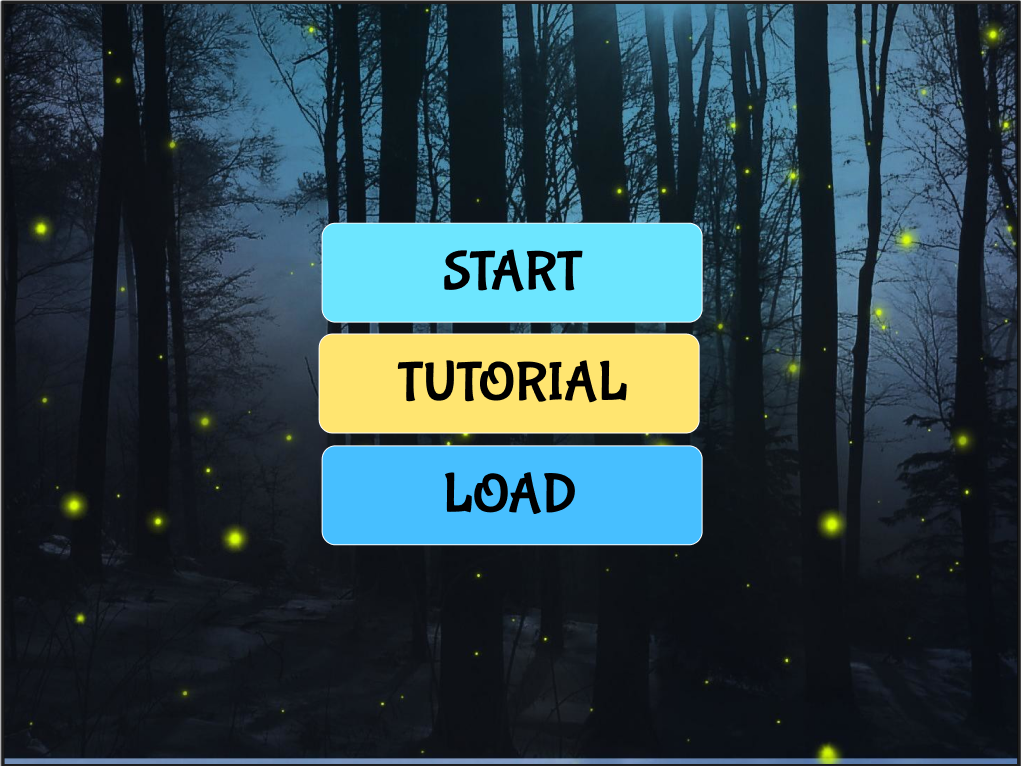
\includegraphics[width=10cm]{figures/MainMenu.png}
    \caption{Main Menu}
    \label{fig:mainmenu}
\end{figure}

The Main Menu (figure \ref{fig:mainmenu}) is the next screen that will show after the splash screen, here the child may tap between 3 buttons, namely: start, tutorial, and load. The start button will open a blank workspace. The tutorial button will show the user how to assemble the firefly step by step and the different gestures that will be utilized. The load button will open the Load Menu where the user may load saved workspaces.

\subsection{Start New}

\begin{figure}[H]
    \centering
    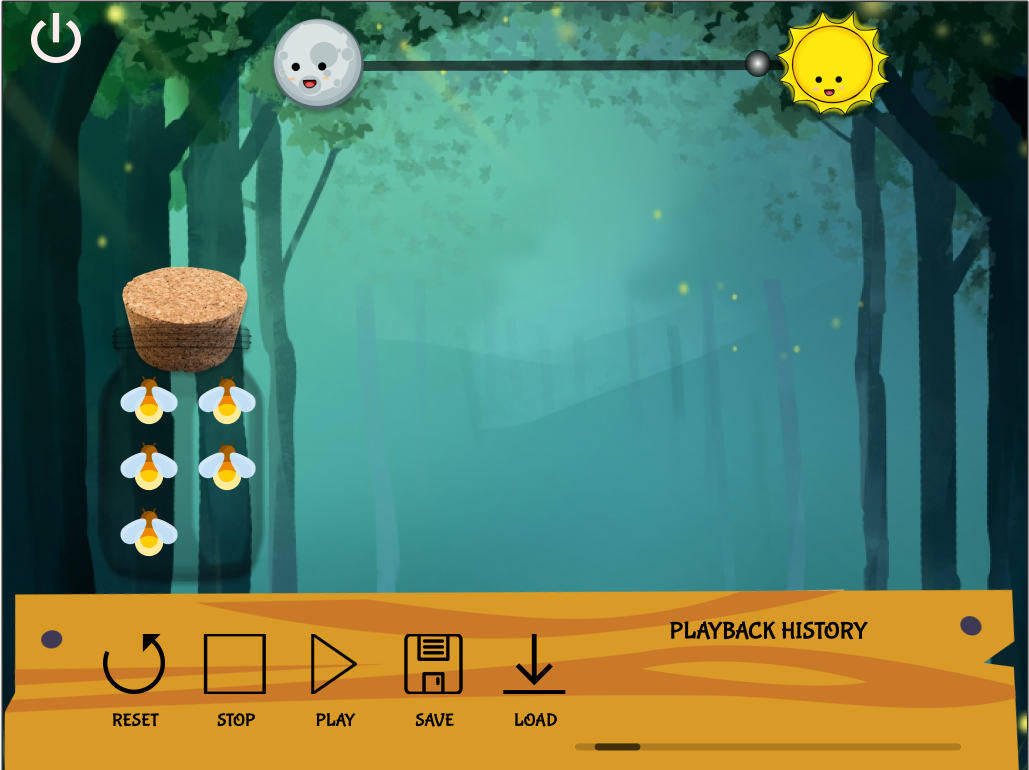
\includegraphics[width=10cm]{figures/BlankSpace.png}
    \caption{Blank Workspace}
    \label{fig:blankworkspace}
\end{figure}

After tapping Start button this is the blank workspace that the child will see figure \ref{fig:blankworkspace}. In this screen, the user will see a jar of fireflies, and other playback controls. This screen is important as this follows the principle of an Obvious Starting point as it becomes a starting point in the application that the child can first explore different interactions and also a safe space for the child as they know that if they commit something wrong they can always go back to this screen.

\subsection{Edit Firefly}

\begin{figure}[H]
    \centering
    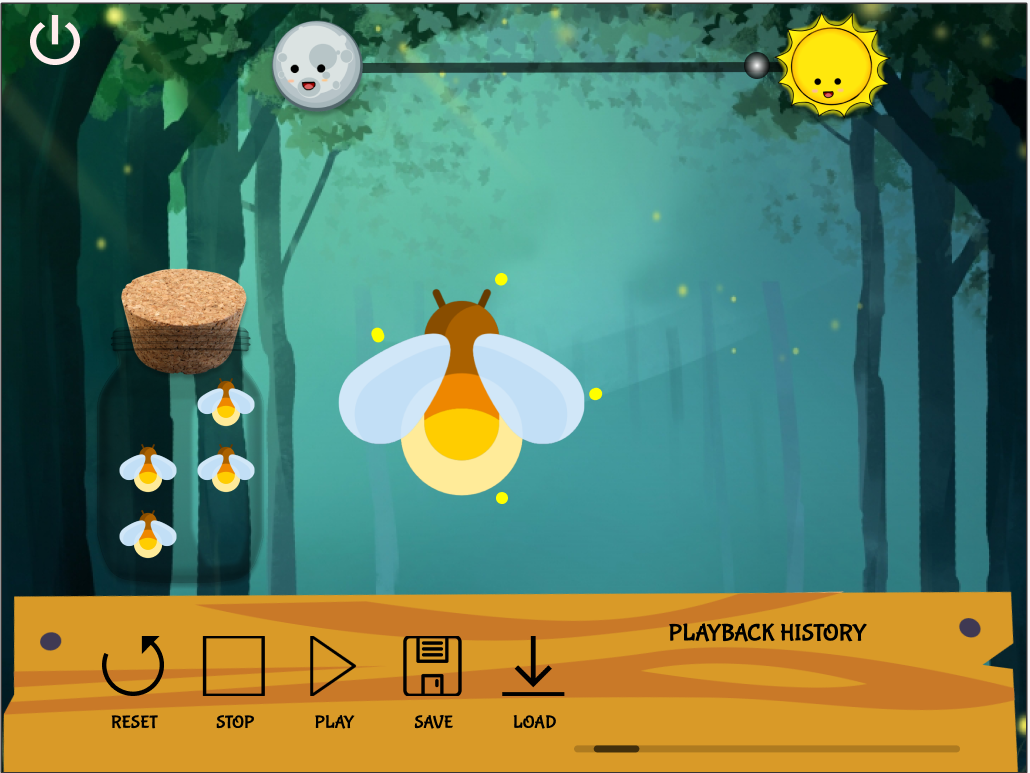
\includegraphics[width=10cm]{figures/ChooseFirefly.png}
    \caption{Editing a Firefly}
    \label{fig:editfirefly}
\end{figure}

After Loading a blank workspace, the child may choose a firefly model to edit by tapping any of the small fireflies in the jar. After tapping a firefly model in the jar, the firefly model will be enlarged so that the child may tap a firefly part to edit. We decided to use simple tap gestures for tasks involved in manipulating the firefly parts to make it easier for the child to remember them and to reduce the load of the actions that can be caused by using other gestures.  

\subsection{Edit Firefly Body}

\begin{figure}[H]
    \centering
    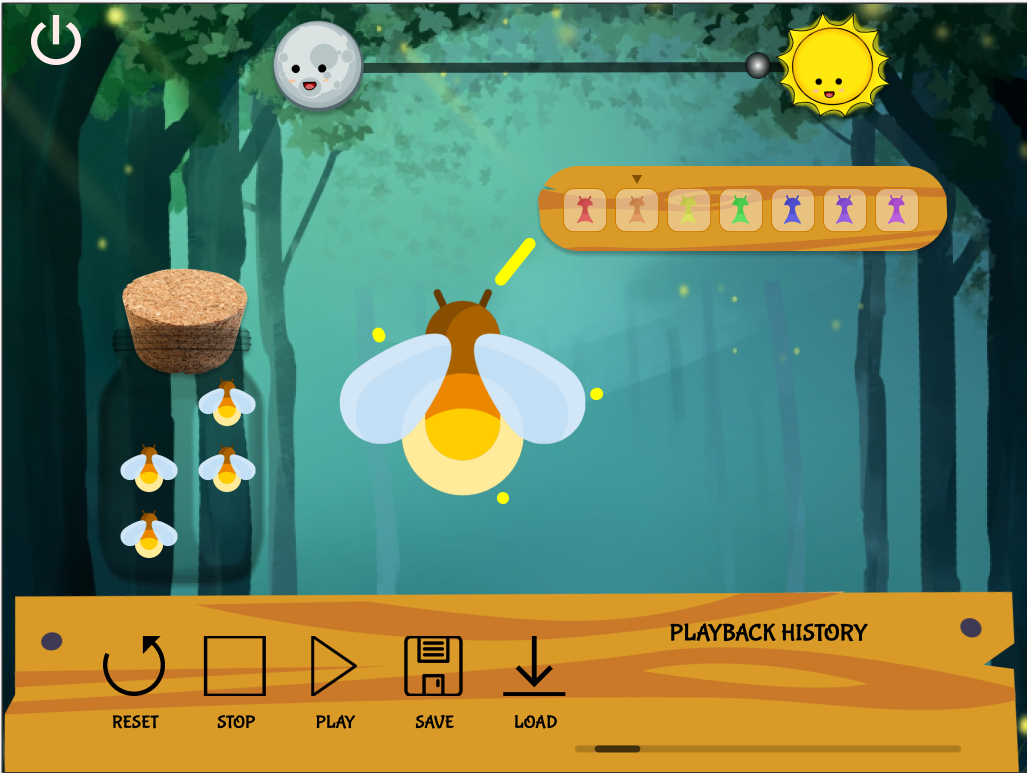
\includegraphics[width=10cm]{figures/Body.png}
    \caption{Editing Firefly Body}
    \label{fig:tweakBody}
\end{figure}

After choosing a firefly model to edit, the child may tap the body to show the popup settings that can configure the properties. The different body color corresponds to different tempos.

\subsection{Edit Firefly Wing}

\begin{figure}[H]
    \centering
    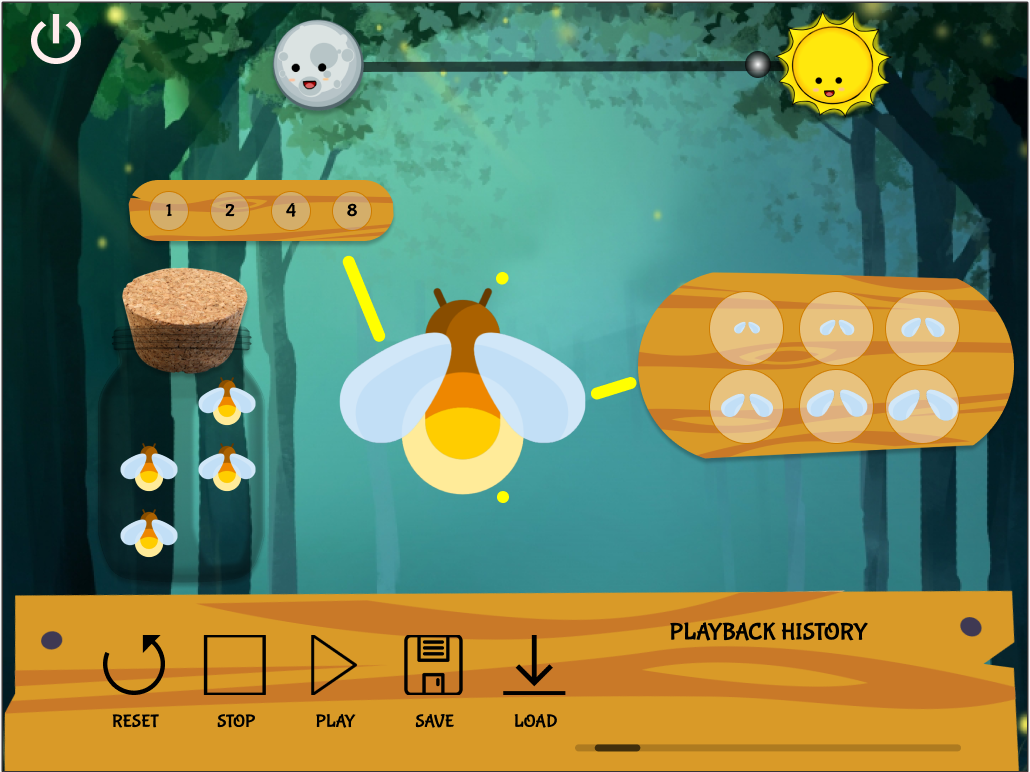
\includegraphics[width=10cm]{figures/Wing.png}
    \caption{Editing Firefly Wing}
    \label{fig:tweakWing}
\end{figure}

After choosing a firefly model to edit, the child may tap the wing to show the popup settings that can configure the properties. For the wing popup settings, there will be two bubbles. The first bubble is for configuring the wing speed. The different wing speed corresponds to length of notes. The other wing configures the wing size. The different wing size corresponds to different number of repetitions. 

\subsection{Edit Firefly Tail Light}

\begin{figure}[H]
    \centering
    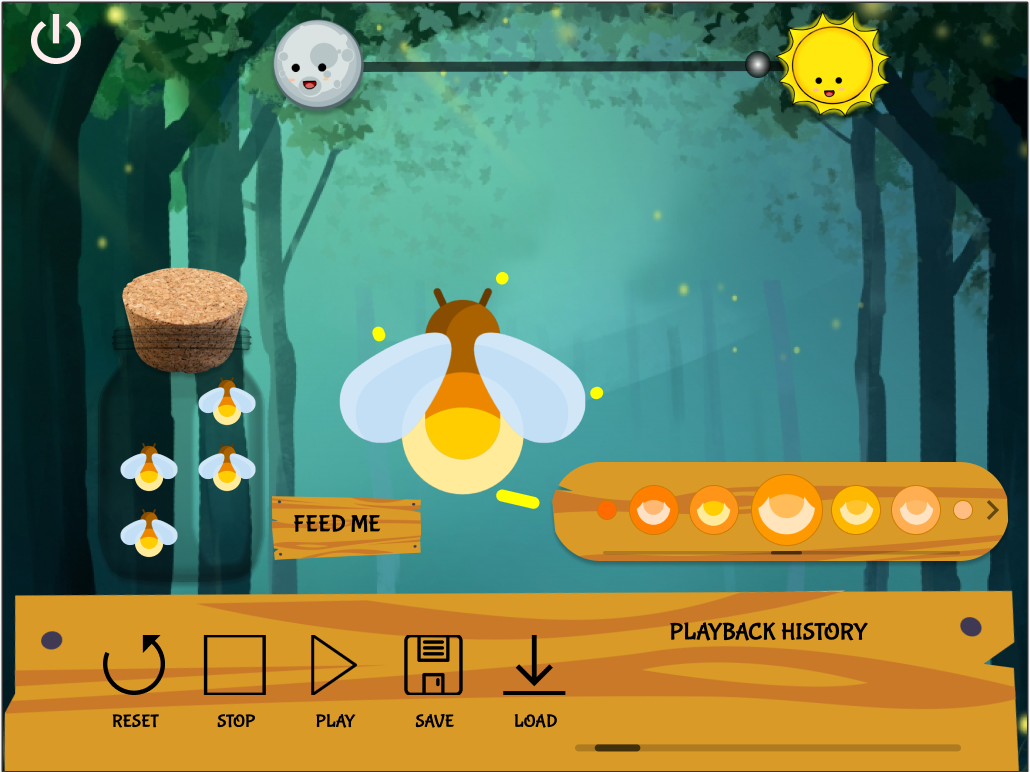
\includegraphics[width=10cm]{figures/Tail.png}
    \caption{Editing Firefly Tail Light}
    \label{fig:tweakTail}
\end{figure}

After choosing a firefly model to edit, the child may tap the tail light to show the popup settings that can configure the properties.

\subsection{Feed Firefly}

\begin{figure}[H]
    \centering
    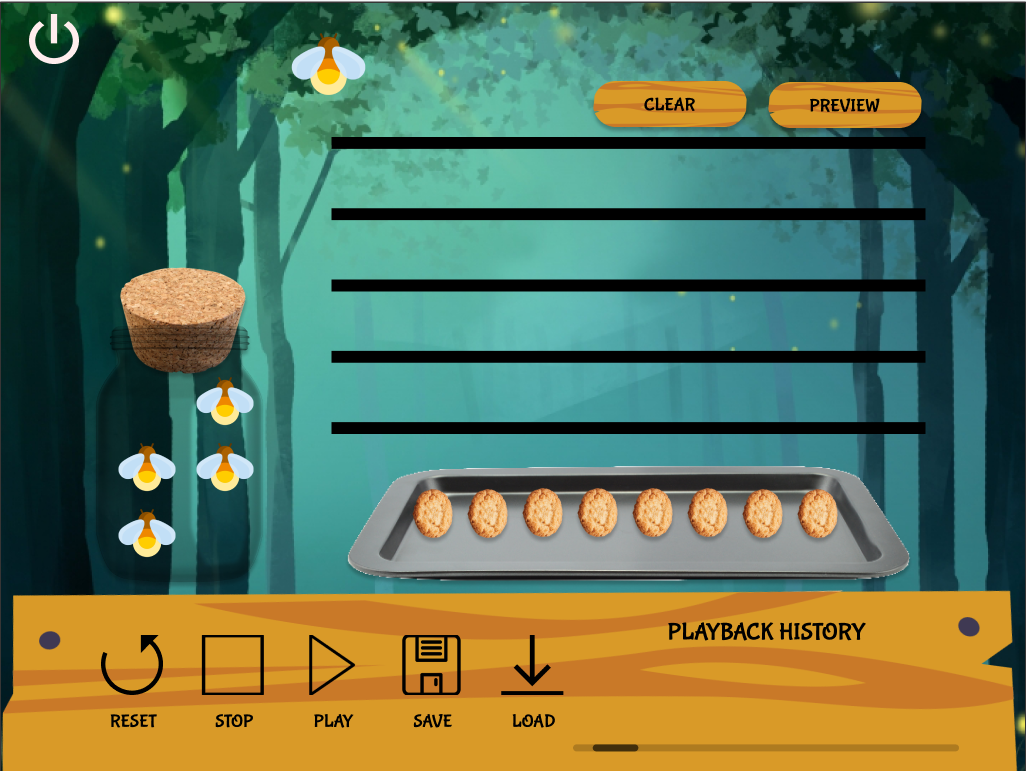
\includegraphics[width=10cm]{figures/FeedFirefly.png}
    \caption{Set Pitch of Notes by Feeding the Firefly}
    \label{fig:feedfirefly}
\end{figure}

After choosing the preferred tail light, the user may tap the feed me button in order to set the biscuits for the path of the firefly model which will also determine the pitch of the notes that the firefly model will play.

\begin{figure}[H]
    \centering
    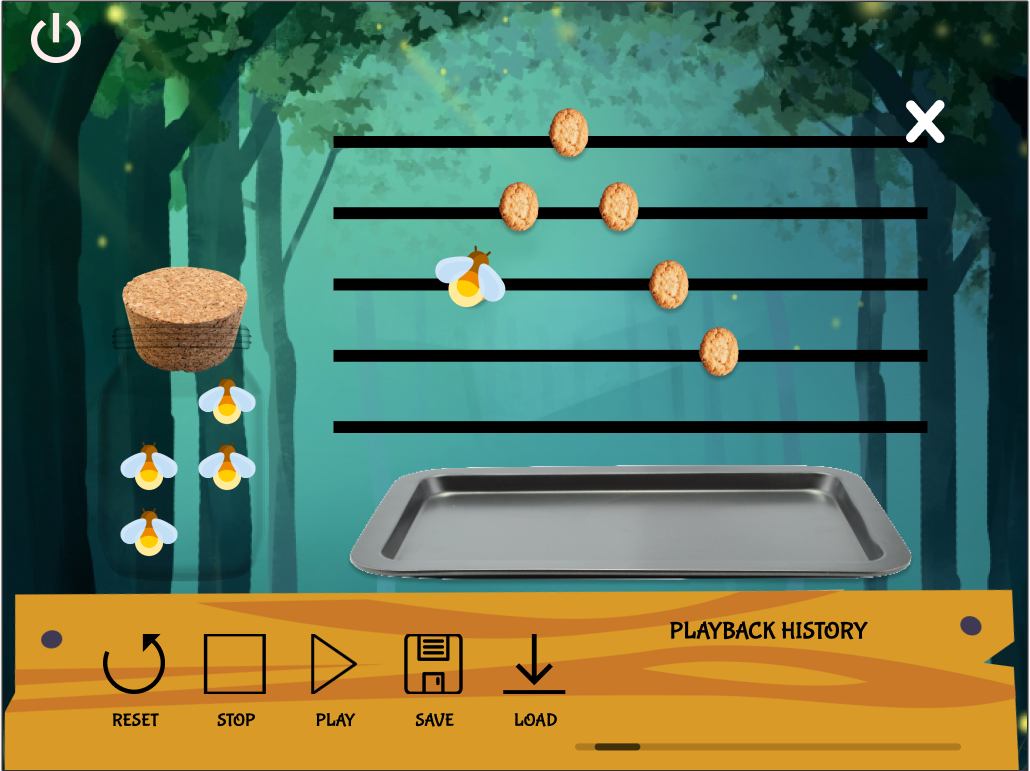
\includegraphics[width=10cm]{figures/PreviewEatingTrail.png}
    \caption{Preview Flight Pattern}
    \label{fig:previewFLight}
\end{figure}

The user may also see a preview of how the firefly model will fly based on their placed biscuits by tapping the preview button.

\subsection{Change Currently editing firefly}

\begin{figure}[H]
    \centering
    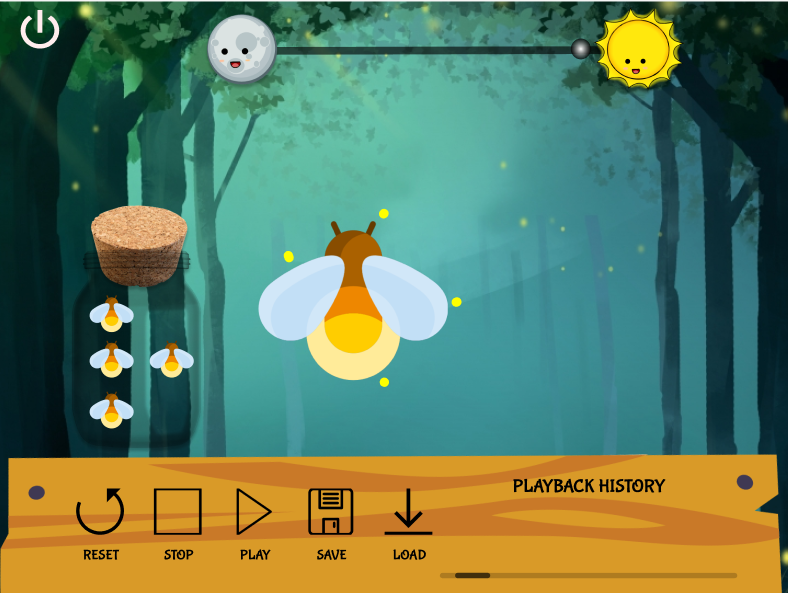
\includegraphics[width=10cm]{figures/ChangeFirefly.png}
    \caption{Choosing Different Firefly to Edit}
    \label{fig:firefly2}
\end{figure}

In order to change the currently editing firefly model to a different firefly model. The child can simply click any of the smaller fireflies to enlarge and the previously enlarged firefly model will minimize. We wanted this action to show a contrast of sizes so that the child focus will shift from the one currently made to the new one.

\subsection{Release Fireflies to start playback}

\begin{figure}[H]
    \centering
    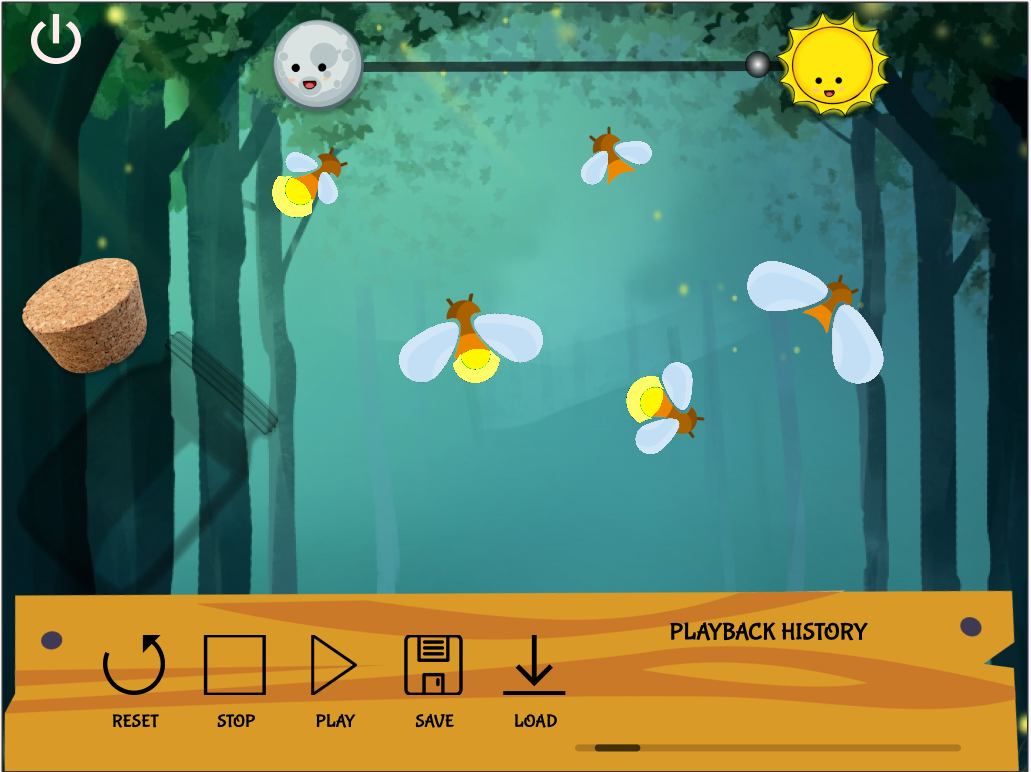
\includegraphics[width=10cm]{figures/Release.png}
    \caption{Releasing the Fireflies}
    \label{fig:releaseFirefly}
\end{figure}

After editing the firefly models to desired configurations, the child can tap on the lid of the jar to release all the fireflies and start the rhythm playback. This particular action was chosen as the start of the playback since we wanted it to represent the real world where fireflies are released and the child can see it as a way of familiarity.

\subsection{Pause, Play, and Stop playback}

\begin{figure}[H]
    \centering
    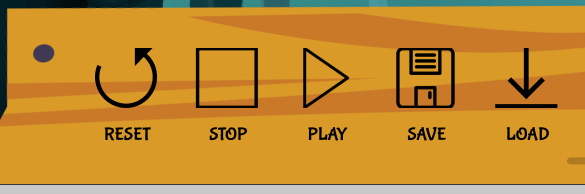
\includegraphics[width=6cm]{figures/StopPlayPause.png}
    \caption{Play Pause, and Stop Controls}
    \label{fig:firefly2}
\end{figure}

During playback, the child can pause and play the playback by toggling the play button. The stop button stops the current playback and starts the playback from the start on pause. The design of the buttons was made to be familiar buttons as they can already give the child an idea of what the buttons do.
 
\subsection{Adjusting Volume}

\begin{figure}[H]
    \centering
    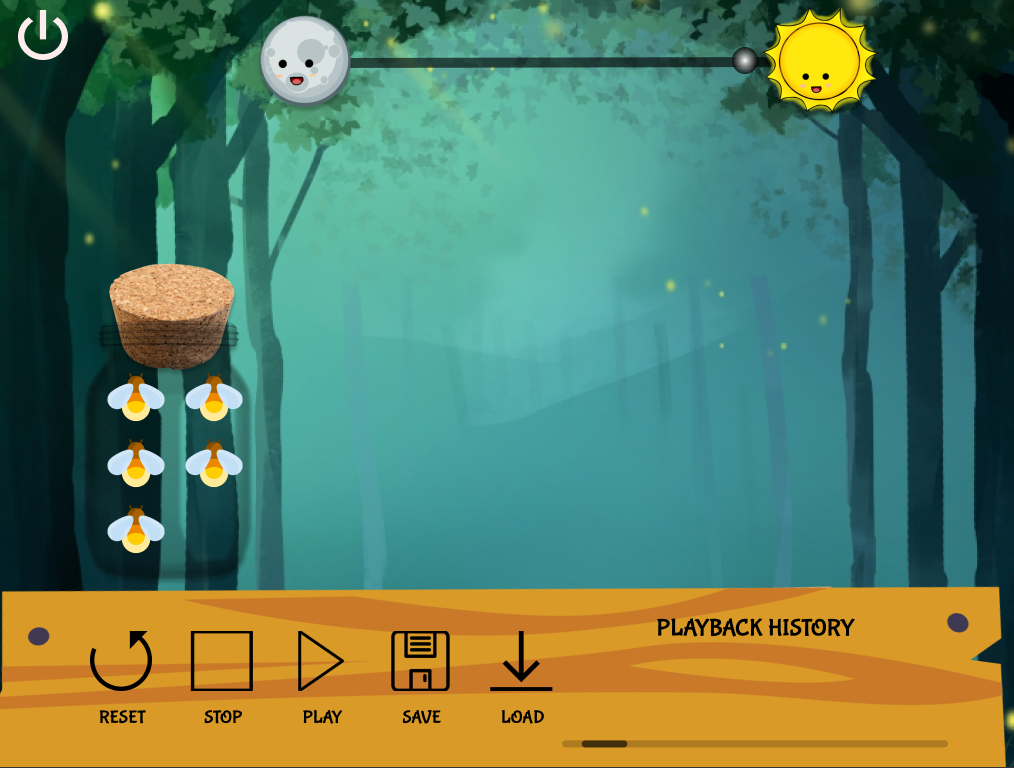
\includegraphics[width=6cm]{figures/volumecontrol.png}
    \caption{Changing Volume of Playback}
    \label{fig:volcontrol}
\end{figure}

During playback, the child can adjust the volume of the playback by using the slider between the sun and moon. The moon will represent a lower volume and the sun will represent a higher volume. One finger drag gesture will be used as the child has more control of the desired volume they need with the use of this gesture.

\subsection{Replay Previous Tracks}

\begin{figure}[H]
    \centering
    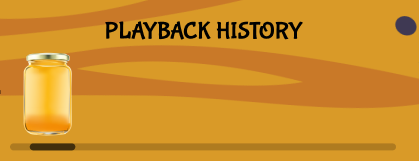
\includegraphics[width=6cm]{figures/historyplayback.png}
    \caption{List of Previous Tracks}
    \label{fig:firefly2}
\end{figure}

After the firefly models are done with their playback, they are placed on to the playback history. The user may play these previous tracks again by dragging them to the jar on the left side then press play. This also was designed to represent the real world action of catching and releasing a firefly.

\subsection{Reset Album}

\begin{figure}[H]
    \centering
    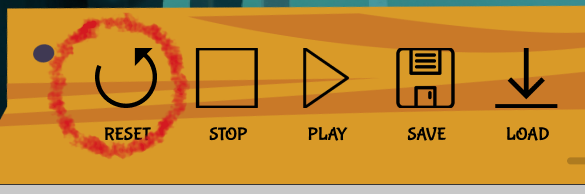
\includegraphics[width=6cm]{figures/resetwork.png}
    \caption{Reset Album Button}
    \label{fig:firefly2}
\end{figure}

If the child wishes to start fresh with a new blank album, the child may press the reset button to return everything to default. We needed to put this as the child can go back to the start which is a screen where he is already familiar with and he would know there is a way to undo their mistakes.

\subsection{Save Album}

\begin{figure}[H]
    \centering
    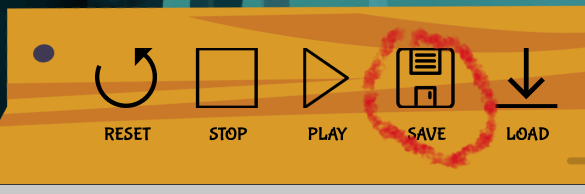
\includegraphics[width=6cm]{figures/Save.png}
    \caption{Save Album Button}
    \label{fig:firefly2}
\end{figure}
The child may choose to save the existing album at anytime. Upon tapping the save button, the child is asked to input an author name and a title for the album. After confirming the album is then saved to the local device and can be loaded at anytime.
\subsection{Load Album}

\begin{figure}[H]
    \centering
    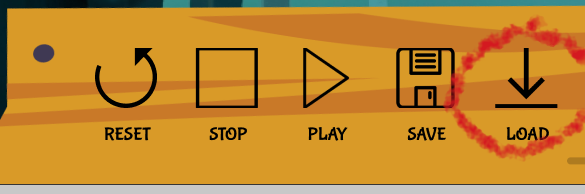
\includegraphics[width=6cm]{figures/load.png}
    \caption{Load Album Button}
    \label{fig:firefly2}
\end{figure}

The child may choose to load an existing album at anytime by tapping the load button.

\subsection{Load Menu}

\begin{figure}[H]
    \centering
    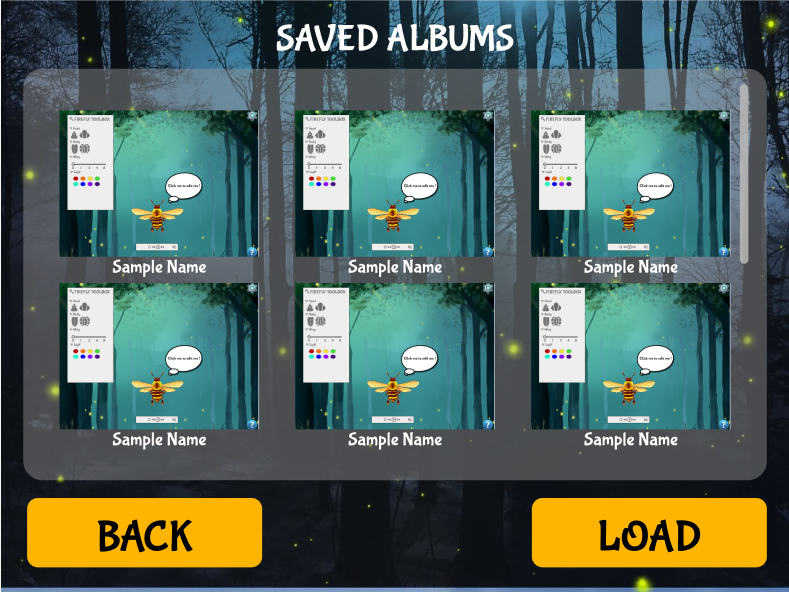
\includegraphics[width=6cm]{figures/LoadMenu.png}
    \caption{Load Menu}
    \label{fig:loadmenu}
\end{figure}

The Load Menu shows all saved albums/workspaces. The child may tap on an album then press the load button to continue working on that album.

\subsection{Exit to Main Menu}

\begin{figure}[H]
    \centering
    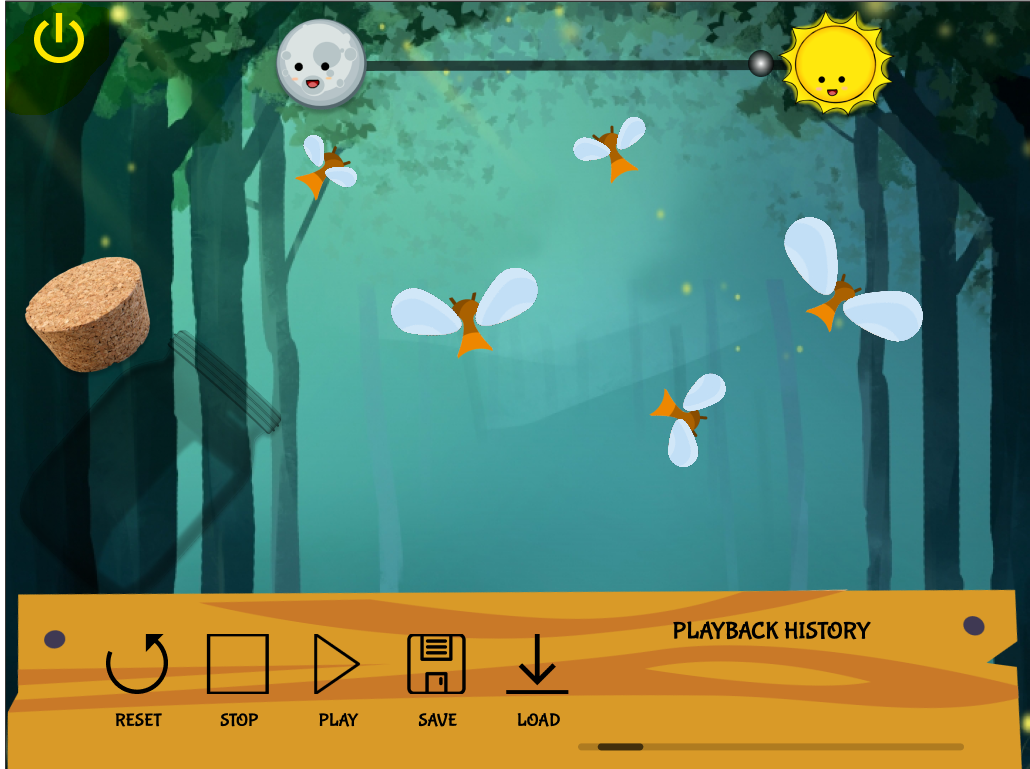
\includegraphics[width=6cm]{figures/exitmenu.png}
    \caption{Exit Button}
    \label{fig:exitbutton}
\end{figure}

The child may choose to tap the exit to main button at any time. When the button is pressed, a confirmation appears and when the child confirms that they want to exit to main menu, the screen will be transferred to the main menu. Same as the start screen this will give the child a sense of relief knowing they can go back to the start and begin all over again.
% \section{Use Case Diagram}
% \begin{figure}[!htb]
%     \centering
%     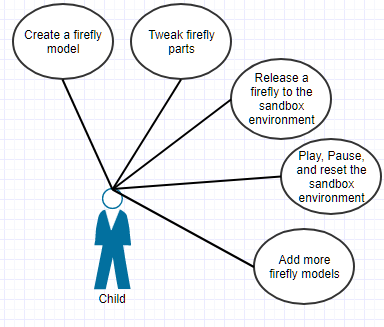
\includegraphics{figures/UseCaseDiagram.PNG}
%     \caption{Use Case Diagram of Firefly}
%     \label{fig:my_label}
% \end{figure}

% This is the use case diagram of Firefly. These are all the actions that the user is allowed to do within the application.

\section{Deployment Plan}
FireflyX will be developed using Xcode using the Swift language. The application once compiled can be uploaded to the Apple App Store where anyone may download the app for free but with in-game purchases. The files will be saved locally this includes the songs and the environment, these files will be exportable with the use of the XML. Using the XML another user in a different iPad can retrieve the same environment by loading the XML sent. A diagram showing the deployment plan is shown in figure \ref{deploymentPlan}.

\begin{figure}[H]
    \centering
    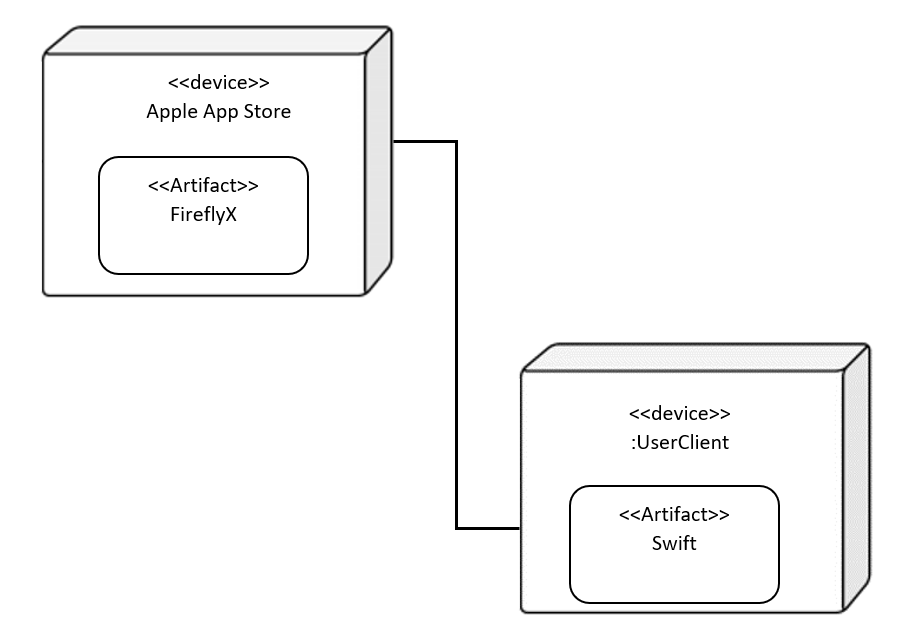
\includegraphics[width=15cm]{figures/deploymentPlan.png}
    \caption{FireflyX Deployment Plan}
    \label{deploymentPlan}
\end{figure}